% ******************************
%* FILE CONFIGURATION
% ******************************
\documentclass[12pt, a4paper]{article}

\usepackage[spanish, es-tabla]{babel} % Enables Spanish language support and table naming
\usepackage{hyperref}                 % Enables creation of hyperlinks in the document
\usepackage{apacite}                  % Enables bibliography management
\usepackage{graphicx}                 % Enables inclusion of images and figures
\usepackage{multirow}                 % Provides multirow functionality for tables
\usepackage{float}                    % Provides better control for floating elements like tables and figures
\usepackage{fancyhdr}                 % Allows customization of headers and footers

% Sets page margins
\usepackage[left=2.5cm, right=2.5cm, top=2cm, bottom=2cm]{geometry}

\pagestyle{fancy}
\fancyhf{}                            % Clears all header and footer fields
\fancyfoot[C]{\thepage}               % Centers the page number at the footer
\renewcommand{\headrulewidth}{0pt}    % Removes the header line
\renewcommand{\footrulewidth}{0pt}    % Removes the footer line

\fancypagestyle{plain}                % Forces the same style on first page
{
  \fancyhf{}
  \fancyfoot[C]{\thepage}
  \renewcommand{\headrulewidth}{0pt}
  \renewcommand{\footrulewidth}{0pt}
}

\setlength{\arrayrulewidth}{0.5mm}    % Adjusts table bstep width
\setlength{\tabcolsep}{5pt}           % Adjusts spacing between table columns

\def\tablename{Tabla}                 % Changes the name of the table caption


% ******************************
%* NEW COMMANDS
% ******************************

% Creates a custom numbered step command (with bold numbers)
\newcounter{step}
\newcommand{\step}[1]
{
  \par\vspace{2ex}
  \stepcounter{step}
  \noindent\textbf{\arabic{step}.} #1\par\vspace{1ex}
}

% Creates a custon numbered step command (without bold numbers)
\newcounter{normalstep}
\newcommand{\normalstep}[1]
{
  \par\vspace{1ex}
  \stepcounter{normalstep}
  \noindent{\arabic{normalstep}.} #1\par\vspace{1ex}
}


% ******************************
%* PSEUDO-CARATULA
% ******************************

\title{TP 3: Redes de Difracción}
\author
{
  Caorsi Juan Ignacio, \href{jcaorsi@itba.edu.ar}{jcaorsi@itba.edu.ar} \\
  Dib Ian, \href{idib@itba.edu.ar}{idib@itba.edu.ar} \\
  Moschini Rita, \href{rmoschini@itba.edu.ar}{rmoschini@itba.edu.ar} \\
  Tamagnini Ana, \href{atamagnini@itba.edu.ar}{atamagnini@itba.edu.ar}
}

\date{Grupo 4 - 27/05/2025}

\begin{document}
\maketitle


% ******************************
%* SECCIONES DEL ARTICULO
% ******************************

\section{Resumen}

En este informe se estudia el fenómeno de difracción e interferencia de la luz utilizando una red de difracción de transmisión. Para ello, 
en el trabajo de laboratorio se iluminó la red con un haz monocromático de láser He-Ne $(\lambda = 632,8$ nm) y con la luz policromática de 
una lámpara de vapor de mercurio.

El primer objetivo fue determinar la constante de red $K$, calculada a partir de la medición de la distancia entre la red y la pantalla y 
de la separación de los máximos de primer orden del patrón de interferencia del láser. El valor obtenido, $K = (5891 \pm 73,9) cm^{-1}$
resulta coherente con el especificado por el fabricante ($K\approx6000\ cm^{-1}$).

A continuación, empleando el valor de $K$ previamente calculado, se midieron las posiciones de los primeros máximos de interferencia 
$(m = \pm 1)$ para las líneas azul, verde y amarillo de la lámpara de mercurio. Las longitudes de onda determinadas fueron:
$\lambda_{azul} = (437,7 \pm 7,6)$ nm, $\lambda_{verde} = (550,6 \pm 8,6)$ nm y $\lambda_{amarillo} = (579,5 \pm 8,9)$ nm. Estos resultados 
concuerdan con los valores teóricos de 436 nm, 546 nm y 577 nm respectivamente, consultados en la bibliografía, ya que todas las 
mediciones caen dentro de sus incertidumbres.


\section{Introducción}

El carácter ondulatorio de la luz se evidencia en fenómenos que no pueden explicarse mediante un modelo basado únicamente en partículas, 
como la interferencia y la difracción \cite{hecht_optics}. Cuando dos o más ondas luminosas se superponen, las variaciones de fase originan zonas de máxima y 
mínima intensidad (interferencia). Por otro lado, al pasar un frente de onda por rendijas o estructuras periódicas, éste se “extiende” más 
allá de la geometría de la abertura, dando lugar a patrones de difracción. Estos efectos fueron estudiados sistemáticamente en el siglo XIX 
y constituyen la base de la óptica moderna.

En el presente trabajo se determina la constante de red $K$ de una malla difractora de transmisión y, con ella, se medirán 
longitudes de onda del espectro del mercurio. Para ello se dispone una fuente láser (He-Ne, $\lambda=632,8$ nm) que ilumina 
perpendicularmente la red, y se registra en una pantalla la posición de los máximos laterales de interferencia. Más adelante, la misma red 
y un arreglo de lente y diafragma se emplean para observar las líneas espectrales de una lámpara de vapor de mercurio.

A continuación, siguiendo el desarrollo de Hecht, partimos de la condición de máximos de interferencia para una red de espaciamiento $d$
y ángulo de difracción $\theta$:
\begin{equation}
  d \,\sin\theta = m \,\lambda
\label{equation1}
\end{equation}

Definiendo la constante de red $K = \frac{1}{d}$ y considerando el primer orden $(m=1)$),  
$\sin\theta = \frac{\lambda}{d}$
$\longrightarrow$
$K = \frac{1}{\lambda}\,\sin\theta$.
Geométricamente, si $Y$ es la mitad de la separación entre los primeros máximos en la pantalla y $D$ la distancia red-pantalla, como se ve 
en la figura \ref{fig1},  
\begin{equation}
  \sin\theta = \frac{Y}{\sqrt{Y^2 + D^2}}
  \quad\Longrightarrow\quad
  K = \frac{1}{\lambda}\,\frac{Y}{\sqrt{Y^2 + D^2}}.
\label{equation2}
\end{equation}

Estas expresiones se emplearán para calcular $K$ con su incertidumbre, y posteriormente, despejando $\lambda$ de la ecuación anterior, 
para obtener las longitudes de onda de las líneas azul, verde y anaranjada del mercurio.


\section{Método Experimental}

Se colocó de forma secuencial una lámpara de vapor de mercurio (la cual emitía un láser de He-Ne), una lente convergente que enfocaba 
la imagen, la red de difracción a estudiar y una pantalla sobre la cual visualizar los máximos de interferencia de primer orden de las 
distintas longitudes de onda.

\subsection{Constante de la red}

Para esta primera parte de la experiencia, se utilizó la pared del laboratorio como pantalla.

Como se observa en la figura 1, con la luz de la lámpara de vapor se iluminó la red de difracción, permitiendo la observación de varios 
puntos luminosos a ambos lados del máximo central correspondientes a los máximos de interferencia. Luego, se midieron la distancia Y entre 
el máximo de primer orden y el de orden cero, y la distancia D entre la pared y la red. Con estas mediciones directas, las ecuaciones 
desarrolladas anteriormente y el dato de que la longitud de onda del haz emitido por el dispositivo es $\lambda = 632,8$ nm, se calculó 
la constante $K$ de la red.

Vale la pena aclarar que, para obtener la distancia Y, se tomó la distancia 2Y entre los máximos de primer orden para tener un menor error 
relativo (al ser mayor el valor medido, su incerteza es menor en comparación). Además, de esta manera se tiene en consideración que la 
pared puede no encontrarse ubicada de forma perfectamente paralela a la red.

\begin{figure}[!h] 
        \centering 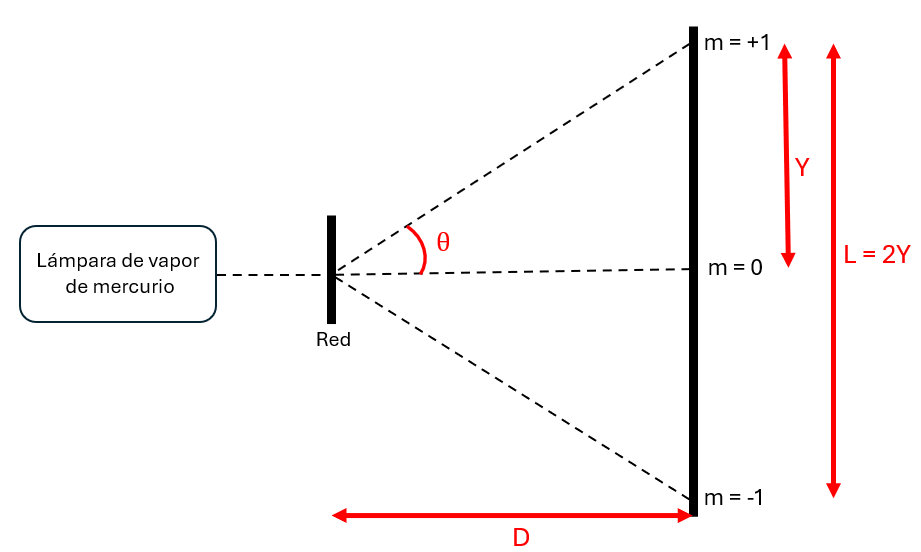
\includegraphics[width=0.9\columnwidth]{diagramaExperimental1.png}
        \caption{\label{fig1}Diagrama de la disposición experimental para calcular la constante de la red, junto con las variables 
        intervinientes.}
\end{figure}

\subsection{Longitud de onda de las líneas azules, verdes y rojas}

En esta segunda parte del experimento, para determinar las longitudes de onda de los distintos componentes del haz emitido por la lámpara 
de mercurio, se armó la disposición experimental igual que se hizo para la primera parte, con la adición de una pantalla blanca en el 
extremo opuesto a la lámpara de vapor, un diafragma contiguo a la lámpara y previo a la red, y una lente convergente contigua al diafragma 
y también previa a la red (ver figura 2).

Se ajustó tanto la cantidad de luz que permitía pasar el diafragma, como su posición y la posición de la lente, de manera que las líneas de 
los máximos de interferencia de primer orden correspondientes a las distintas longitudes de onda se vieran con la mayor nitidez posible y 
sean a la vez lo más finas posibles (para obtener mediciones más precisas). 

Finalmente, se midieron la distancia D entre la pantalla y la red, y las distancias $2Y_{azul}$, $2Y_{verde}$ y $2Y_{naranja}$ entre los 
máximos de primer orden de cada color (es decir, de cada longitud de onda).

\begin{figure}[!h] 
        \centering 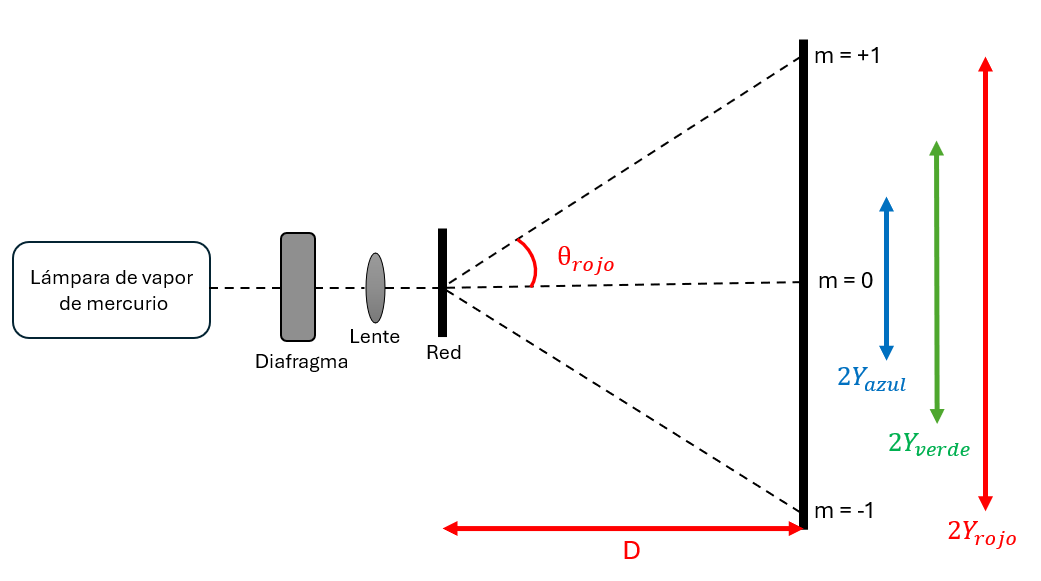
\includegraphics[width=0.9\columnwidth]{diagramaExperimental2.png}
        \caption{\label{fig2}Diagrama de la disposición experimental para calcular las longitudes de onda, junto con las variables 
        intervinientes.}
\end{figure}

\begin{figure}[!h] 
        \centering 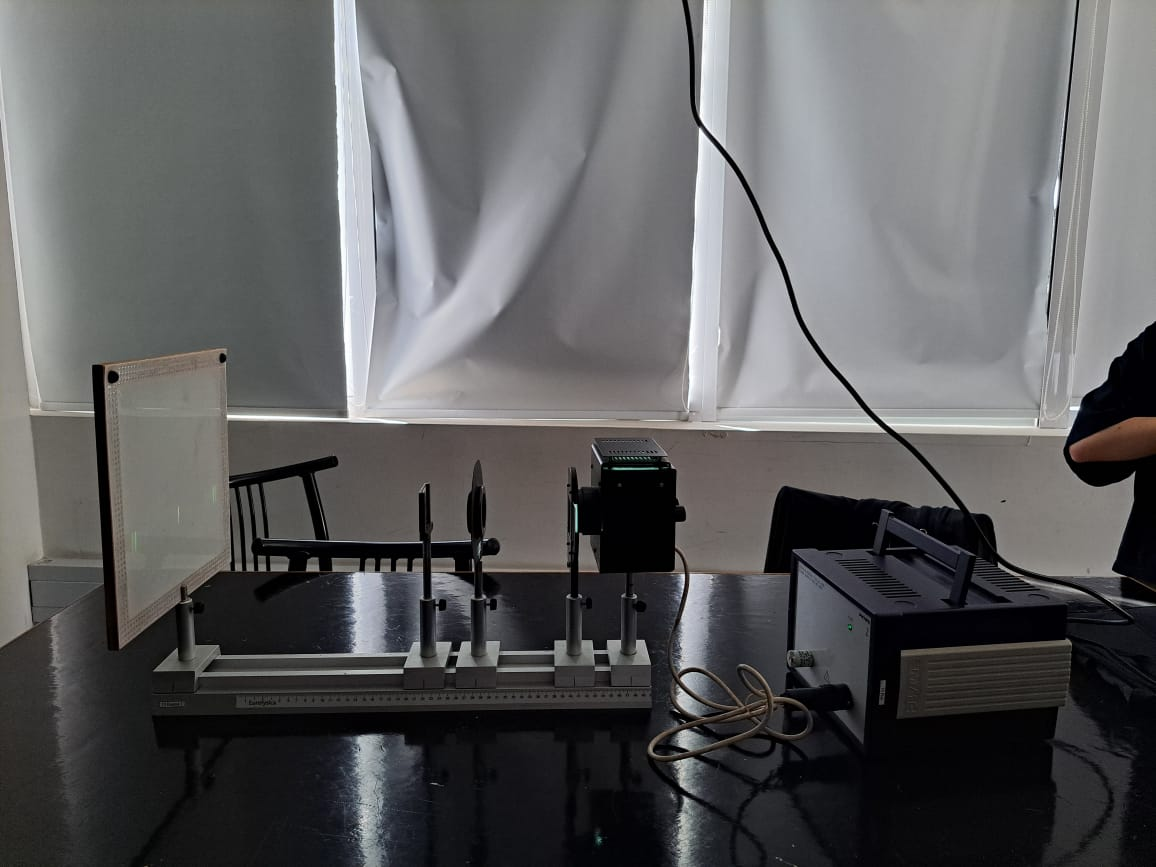
\includegraphics[width=0.75\columnwidth]{dispositivo3.jpg}
        \caption{\label{fig3}Foto de la disposición experimental en funcionamiento. De derecha a izquierda se pueden ver la fuente de 
        alimentación, la lámpara de vapor de mercurio, el diafragma, la lente, la red de difracción y la pantalla.}
\end{figure}

\newpage
\section{Resultados}

\subsection{Constante de la red}
Se midieron los valores $D = (169 \pm 0,1)$ cm y $2Y = (139,40 \pm 1)$ cm. Reemplazando en la ecuación \ref{equation2},  se obtiene 
$K = (5891 \pm 73,9) cm^{-1}$.

\subsection{Longitud de onda de las líneas azul, verde y roja}
Se midieron el valor $D = (29,6 \pm 0,1)$ cm y los valores de Y presentados en la siguiente tabla:

\begin{table}[H]
  \centering
  \begin{tabular}{|c|c|}
  \hline
  Color & Y (cm) \\
  \hline
  $Azul$  & $7,9 \pm 0,1$  \\ \hline
  $Verde$  & $10,15 \pm 0,1$ \\ \hline
  $Amarillo$  & $10,75 \pm 0,1$ \\ \hline
  \end{tabular}
  \caption{\centering Valores de las distancias entre el máximo de primer orden y el de orden cero de cada longitud de onda (Y, no 2Y).}
  \label{tabla1}
\end{table}

Reemplazando en la ecuación \ref{equation2} se obtienen las longitudes de onda presentadas en la siguiente tabla:

\begin{table}[H]
  \centering
  \begin{tabular}{|c|c|}
  \hline
  Onda por color & $\lambda $ (nm)  \\
  \hline
  ${\lambda_{azul}}$  & $ 437,7 \pm 7,6$  \\ \hline
  ${\lambda_{verde}}$  & $ 550,6 \pm 8,6 $ \\ \hline
  ${\lambda_{amarillo}}$  & $ 579,5 \pm 8,9 $\\ \hline
  \end{tabular}
  \caption{\centering Valores calculados de las longitudes de onda de tres colores. }
  \label{tabla2}
\end{table}


\section{Conclusiones}

En la primera parte del experimento se obtuvo que la constante de la red es  $K = (5891 \pm 73,9) cm^{-1}$, valor que resulta razonable al 
compararlo con la especificación del fabricante $(K\approx6000\ cm^{-1})$. Se estima que el error relativo de 1,25\% proviene de la 
determinación de la posición de los máximos y de la medición de la distancia red-pantalla.

Para las longitudes de onda de las líneas del mercurio se hallaron $\lambda_{azul} = (437,7 \pm 7,6)$ nm, 
$\lambda_{verde} = (550,6 \pm 8,6)$ nm y $\lambda_{amarillo} = (579,5 \pm 8,9)$ nm. Al comparar estos valores experimentales con los teóricos 
(436 nm, 546 nm y 577 nm respectivamente \cite{uiowa_mercury}), se observó que se encuentran dentro del rango de las incertidumbres 
experimentales. Las desviaciones relativas menores al 2\% pueden atribuirse a factores como la alineación imperfecta del montaje y la 
resolución limitada en la medición de la separación entre máximos.


\section{Apéndice: Cálculo de Incertezas}

\subsection{Constante de la red}
Dado que en esta primera parte la longitud de onda del haz emitido se considera como dato (un valor exacto), entonces su incerteza 
$\Delta \lambda$ es nula y ${\Delta}K$ se calcula como:

\begin{equation}
  {\Delta}K = \sqrt{({\Delta}y)^2(\frac{D^{2}}{{\lambda} \left(Y^{2} + D^{2}\right)^{\frac{3}{2}}})^2+({\Delta}D)^2(-\frac{YD}
  {{\lambda} \left(D^{2} + Y^{2}\right)^{\frac{3}{2}}})^2}
\label{equation3}
\end{equation}

donde $\Delta y = \frac{\Delta L}{2}$ y, como los máximos de interferencia no son puntuales, tomamos $\Delta L \approx 2$ cm correspondiente
al diámetro del punto de luz.

\subsection{Longitud de onda de las líneas azul, verde y roja}
En esta segunda parte, sabemos que $\Delta D = 0,1$ cm.

Para calcular la incerteza de cada longitud de onda utilizamos la siguiente ecuación:
\begin{equation}
  {\Delta}{\lambda} = \sqrt{({\Delta}K)^2(-\frac{Y}{\sqrt{Y^{2} + 
  D^{2}} \, K^{2}})^2 + ({\Delta}D)^2(-\frac{YD}{K \left(D^{2} + Y^{2}\right)^{\frac{3}{2}}})^2+({\Delta}Y)^2(\frac{D^{2}}{K \left(Y^{2} 
  + D^{2}\right)^{\frac{3}{2}}})^2}
\label{equation4}
\end{equation}

Se pueden ver los valores de cada longitud de onda junto a su respectiva incerteza en la tabla \ref{tabla2}, en la sección de resultados.

\newpage
\bibliographystyle{apacite}           % Follows APA style
\bibliography{bibliography}           % File with the bibliography info.


\end{document}
